\chapter{Contexte mathématique}

	\section{Introduction}

	L’introduction de l’obligation pour les banques de se prémunir contre d’éventuelles pertes financières a naturellement entraîné l’utilisation de différents concepts mathématiques. En effet, pour les banques, l’enjeu est d’immobiliser le minimum de ressources financières, tout en garantissant un niveau de risque satisfaisant. Il est donc naturel que des notions de statistiques et de probabilités soient introduites afin quantifier le risque. Contextees notions sont présentées par la suite.


	\section{Définitions}

		Pour pouvoir quantifier le risque, il faut tout d’abord modéliser les variations des valeurs boursières. Pour cela, on utilise des séries temporelles. Une série temporelle est une suite de valeurs numériques représentant l'évolution d'une quantité au cours du temps. La valeur de $x$ à l’instant $t$ sera ainsi notée $x_t$. L’introduction de la notion de temps doit être accompagnée de la définition d’une unité de temps. Dans notre cas, l’unité de temps est le jour. Si nous sommes à l’instant $t$, $t-1$ correspond à la veille et $t+1$ au lendemain.

		Pour estimer les risques financiers, différentes techniques existent. L'une des plus utilisées actuellement est la Value-at-Risk (VaR). Elle permet de mesurer les risques associés à un \gls{portefeuille}.
		Plus précisement, elle permet d'estimer la perte maximale associée à un portefeuille pour un niveau de confiance et un horizon de temps donnés. Elle peut être calculée selon plusieurs méthodes. Nous en présentons trois par la suite.\\
		On définit $V_t$ comme le prix de vente du \gls{portefeuille} à l'instant t. Le log-rendement correspond au logarithme du rapport de deux prix de vente successifs :
		$r_t = \log\left(\frac{V_t}{V_{t-1}}\right)$


	\section{Particularités statistiques des séries financières}

		La modélisation des séries financières est particulièrement complexe car celles-ci ont des comportements atypiques.

		\begin{figure}[h]
			\center
			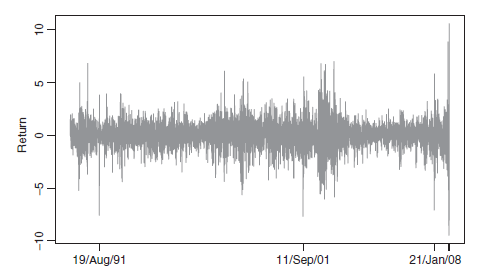
\includegraphics{logRendementCAC40.png}
			\caption{Log rendement du CAC 40 entre 1990 et 2008}
			\label{log_rendement}
		\end{figure}

		Tout d'abord, les valeurs extrêmes ont tendance à se regrouper; on parle alors de \textit{Volatility clustering}. En effet, lorsque les cours sont instables, la probabilité qu'ils le soient le lendemain est assez élevée; de même lorsqu'ils sont stables, ils ont plus tendance à le rester.
		De plus, les queues de distributions des rendements sont épaisses. Cela signifie que les valeurs extrêmes ont une probabilité non négligeable d'apparaître. Cela est donc plus compliqué à modéliser : les rendements ne suivent pas une loi normale par exemple.
		Un autre effet qui peut compliquer la modélisation est l'effet de levier. Cet effet correspond au fait qu'une même variation des cours n'aura pas la même conséquence, suivant qu'elle soit positive ou négative. En effet, une baisse des cours entrainera une instabilité plus importante qu'une variation positive de même amplitude. L'influence de la variation des rendements n'est donc pas symétrique.
		Enfin, une certaine saisonnalité des rendements est parfois observée. En effet, suivant la période de l'année ou suivant le jour, ils seront plus ou moins volatiles.
		Il n'existe pas à ce jour de modèle permettant de modéliser l'ensemble de ces particularités. Mais comme celles-ci n'ont pas toutes la même importance, des modèles plus simples permettent de modéliser correctement l'évolution des rendements financiers.
		
		Il faut également noter qu'il existe d'autres particularités (corrélation entre les différentes actions notamment) mais elles ne sont pas expliquées ici car elles ne seront pas prises en compte dans notre logiciel.


	\section{Modèle GARCH}

		%\subsection{Le Modèle ARCH}
		%Afin de modéliser l'évolution des rendements, différents modèles ont été introduits. Le modèle le plus simple est le modèle ARCH.
		%Il est défini par deux équations : 
		%\[r_t = \sigma_t\eta_t , \eta_t~iid(0,1)\]
		%\[\sigma_t^2 = \omega+\sum_{i=1}^n \alpha_i*r_{t-i}^2\]

		%La première équation modélise le fait que le rendement s'exprime comme le produit d'une variance $\sigma_t$ (calculée à partir des observations précédentes) avec une variable aléatoire $\eta_t$. Cette variable aléatoire permet de modéliser les évènements imprévisibles.

		%La seconde équation porte sur le calcul de la variance. Ce calcul est ici effectué par rapport aux rendements précédents. Les $\alpha_i$ sont présents afin de moduler l'influence des rendements en fonction de leur éloignement par rapport à la date actuelle. Ainsi, les rendements les plus récents auront un poids plus élevé que les rendements plus anciens. Néanmoins, ce modèle ne prend pas vraiment en compte certaines spécificités. Par exemple, il a été remarqué que lorsque les rendements varient peu, les futurs rendements varient peu également (et vice versa s'il y a beaucoup de variations). Ainsi, ce modèle a été complété afin de prendre en compte cette information.


		\subsection{Le modèle GARCH}
		\label{subsubsection:modele-garch}
			Afin de modéliser l'évolution des rendements, différents modèles ont été introduits. Un des modèles les plus utilisés est le modèle GARCH.
			Il est défini par deux équations :

			\[r_t = \sigma_t\eta_t , \eta_t~iid(0,1)\]
			\[\sigma_t^2 = \omega+\alpha*r_{t-1}^2+\beta*\sigma_{t-1}^2\] avec $\omega, \alpha, \beta > 0$

			La première équation modélise le fait que le rendement s'exprime comme le produit d'une variance $\sigma_t$ (calculée à partir des observations précédentes) avec une variable aléatoire $\eta_t$. Cette dernière quantité permet de modéliser les évènements imprévisibles.

			La seconde équation porte sur le calcul de la variance. Ce calcul est effectué par rapport aux rendements et aux variances précédents. Les $\alpha$ et $\beta$ sont présents afin de moduler l'influence des informations (rendements et variances).

			Le modèle GARCH présenté ici est assez simple et il en existe d'autres prenant en compte des données plus anciennes que celles obtenues au temps $t-1$. Il permet néanmoins de bien modéliser le \textit{Volatility clustering}. En revanche, il ne tient pas compte de l'asymétrie de la variation des rendements. Il existe donc d'autres modèles, basés sur le GARCH, qui permettent de mieux modéliser certaines particularités de séries financières.

			\begin{figure}[h]
				\center
				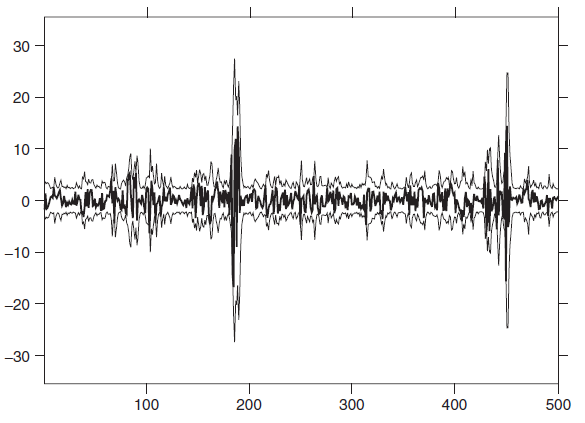
\includegraphics{AjustementParGarch.png}
				\caption{Exemple de prévision par un modèle GARCH}
				\label{ajustement_garch}
			\end{figure}


		\subsection{Conditions d'application du modèle GARCH}
		\label{subsubsection:condition-garch}
			Comme tout modèle, GARCH doit être appliqué sous certaines conditions. Tout d'abord, il est nécessaire de vérifier qu'il n'existe pas de corrélation entre les rendements à des temps différents.
			%\[\mathbb{E}(r_{t})=\mathbb{E}(\sigma_{t})*\underbrace{\mathbb{E}(\eta_{t})}_{=0}=0\]
			%\begin{align}
			%\operatorname{cov}(r_{t},r_{t-1})
			%&=\mathbb{E}(r_{t}*r_{t-1})-\underbrace{\mathbb{E}(r_{t-1})}_{=0}*\underbrace{\mathbb{E}(r_{t})}_{=0}\\
			%&=\mathbb{E}(r_{t}*r_{t-1}) \\
			%&= \mathbb{E}(\sigma_t*\sigma_{t-1})*\underbrace{\mathbb{E}(\eta_t)}_{=0}*\underbrace{\mathbb{E}(\eta_{t-1})}_{=0} = 0
			%\end{align}
			Pour cela on calcule, à partir des données collectées, la covariance empirique et on teste sa nullité. 

			Une autre condition est que la covariance calculée à partir des rendements au carré soit supérieure à zéro.
			%\begin{align}
			%\operatorname{cov}(r_{t}^{2},r_{t-1}^{2})
			%&=\mathbb{E}(\sigma_t^2*\sigma_{t-1}^2)*\underbrace{\mathbb{E}(\eta_t^2)}_{=1}*\underbrace{\mathbb{E}(\eta_{t-1}^2)}_{=1}\\
			%&=\mathbb{E}((\omega+\alpha*r_{t-1}^2+\beta*\sigma_{t-1}^2)\sigma_{t-1}^2)\\
			%&=\omega*\mathbb{E}(\sigma_{t-1}^{2})+\alpha*\mathbb{E}(r_{t-1}^2*\sigma_{t-1}^2)+\beta*\mathbb{E}(\sigma_{t-1}^4)\\
			%&=\omega*\underbrace{\mathbb{E}(\sigma_{t-1}^{2})}_{>0}+\alpha*\underbrace{\mathbb{E}(\sigma_{t-1}^4)}_{>0}+\beta*\underbrace{\mathbb{E}(\sigma_{t-1}^4)}_{>0}
			%&>0
			%\end{align}
			Pour vérifier cela, on calcule, à partir des données collectées, la covariance empirique des rendements au carrés et on vérifie sa positivité.

			Toutes ces différentes conditions sont basées sur des résultats théoriques et elles peuvent également être vérifiées en traçant différents graphiques.

			Il existe encore d'autres conditions d'applications (notamment sur les valeurs des $\alpha$ et $\beta$), mais celles-ci ne seront pas abordées ici car elles sont plus complexes.


		\subsection{Lien avec la Value at Risk}
			La modélisation GARCH nous permet ainsi de modéliser l'évolution des rendements. Il nous faut maintenant lier ces rendements à la VaR.
			Par définition, on a :
			\[\alpha = \mathrm{P}(VaR_{t,h}(\alpha)\textless (V_t - V_{t+h})) si V_{t+h} < V_t. Sinon, VaR_{t+h} = 0\]
			Cela exprime bien le fait que la probabilité que la valeur de la perte ($V_t - V_{t+h}$) dépasse la VaR vaut $\alpha$.
			
			Si on développe cette expression on obtient : 
\begin{align}
\alpha &= \mathrm{P}(VaR_{t,h}(\alpha)\textless -(V_{t+h} - V_t))\\
			&= \mathrm{P}\left(\frac{-VaR_{t,h}(\alpha)}{V_t}\textgreater\frac{(V_{t+h} - V_t)}{V_t}\right)\\
			&= \mathrm{P}\left(1-\frac{VaR_{t,h}(\alpha)}{V_t}\textgreater\frac{V_{t+h}}{V_{t+h-1}}*\frac{V_{t+h-1}}{V_{t+h-2}}*...*\frac{V_{t+1}}{V_{t}}\right)\\
			&= \mathrm{P}\left(\log (1-\frac{VaR_{t,h}(\alpha)}{V_t})\textgreater r_{t+h}+r_{t+h-1}+r_{t+h-2}+...+r_{t+1}\right)
\end{align}

			On arrive donc à montrer que $VaR_{t+h}(\alpha) = 1 - exp{(q_{t}(h,\alpha))}*V_{t}$, avec $q_{t}(h,\alpha)$ le quantile d'ordre $\alpha$ de $r_{t+h}+r_{t+h-1}+r_{t+h-2}+...+r_{t+1}$. On voit donc ici que la VaR est caluclée à partir de rendements futurs et donc encore non observés. Il est donc nécessaire d'estimer ces rendements à l'aide d'un modèle GARCH bien ajusté aux données observées.
	
	\section{Calcul de la Value at Risk}

		\subsection{Par la méthode historique}
		\label{subsubsection:methode-historique}
			Historiquement, la VaR se calcule à partir de l'histogramme des rendements. En effet, la méthode originale consiste à prendre la valeur limite correspondant à un certain pourcentage des rendements les plus faibles. Le risque $\alpha$ évoqué précédemment est alors ce pourcentage. Cela revient donc à prendre le quantile d'ordre $\alpha$ de la distribution de la valeur du portefeuille.


		\subsection{Par la méthode RiskMetrics}
		\label{subsubsection:methode-riskmetrics}
			L'une des méthodes les plus utilisées pour estimer la VaR est la méthode RiskMetrics. Elle correspond à un modèle GARCH particulier. En effet, avec RiskMetrics, la valeur de la variance est calculée uniquement par rapport aux données obtenues au temps $t-1$, dans notre cas la veille. De plus, la somme des coefficients $\alpha$ et $\beta$ est égale à 1. Enfin, le terme constant de variance ($\omega$) est nul. On a donc le modèle suivant :
			\[r_t = \sigma_t\eta_t , \eta_t~iid(0,1)\]
			\[\sigma_t^2 = (1-\lambda)*r_{t-1}^2+\lambda*\sigma_{t-1}^2\]

			L'avantage de cette méthode simplifiée est que le calcul de la VaR est direct. Ce modèle, bien qu'il ne soit pas le plus fiable, est néanmoins très utilisé, grâce à sa simplicité.

			Contrairement au modèle GARCH, la valeur de l'unique coefficient $\lambda$ n'est pas calculée avec les données précédentes. En effet, il est souvent fixée à une valeur, obtenue par expérience, de $0.94$.


		\subsection{Par la méthode bootstrap}
		\label{subsubsection:methode-bootstrap}
			En dehors des deux méthodes précédentes, le calcul de la VaR ne peut se faire de façon directe. En effet, comme précisé plus haut, le calcul de la VaR dépend d'un quantile d'une loi inconnue\footnote{La loi de la somme des rendements n'est pas connue à priori}. Comme ce quantile ne peut être déterminé de façon théorique, il doit être estimé. Cette estimation est réalisée par la méthode \textit{bootstrap}. Cette méthode consiste à générer un grand nombre scénarios et à calculer la somme des rendements pour chacun d'entre eux. Ainsi, on obtient un nombre assez important de sommes de rendements. Comme ces sommes suivent la loi inconnue que l'on cherche pour calculer la VaR, on peut les utiliser pour obtenir le quantile qui nous intéresse (soit directement, soit en cherchant à estimer la fonction de densité).

			Cependant, pour que la loi obtenue par les scénarios soit pertinente, ces scénarios sont générés à partir de données déjà observées. De ce fait, la première étape du \textit{bootstrap} consiste à calculer les résidus $\eta_t$ sur des données observées. Ensuite, on réalise un tirage avec remise entre les différents résidus pour générer les scénarios. Lorsque l'on a tiré aléatoirement un résidu, on peut calculer le rendement associé ainsi que la volatilité à l'étape suivante. En répétant ces étapes, on obtient donc différents scénarios(TODO : image scenario).